\documentclass[air,article,submit,moreauthors]{Definitions/mdpi}

\firstpage{1}
\makeatletter
\setcounter{page}{\@firstpage}
\makeatother
\pubvolume{1}
\issuenum{1}
\articlenumber{0}
\pubyear{2026}
\copyrightyear{2026}
\datereceived{ }
\daterevised{ }
\dateaccepted{ }
\datepublished{ }

\Title{Supplementary Material: WRF Cold-Pool Sensitivities Relevant to Winter-Ozone Modelling in the Uinta Basin}

\newcommand{\orcidauthorA}{0000-0003-0305-4090}
\newcommand{\orcidauthorB}{0009-0009-9083-6568}
\Author{John R. Lawson $^{1,2,}$*\orcidA{}, Michael J. Davies $^{1}$\orcidB{}, Loknath Dhar $^{1,3}$ and Seth N. Lyman $^{1,3}$}
\AuthorNames{John R. Lawson, Michael J. Davies, Loknath Dhar and Seth N. Lyman}

\address{%
$^{1}$ \quad Bingham Research Center, Utah State University, Vernal, UT 84078, USA;\\
$^{2}$ \quad Department of Mathematics and Statistics, Utah State University, Logan, UT 84322, USA;\\
$^{3}$ \quad Department of Chemistry and Biochemistry, Utah State University, Logan, UT 84322, USA}
\corres{Correspondence: john.lawson@usu.edu}

\begin{document}

\section{Secondary Controlled Comparisons}
\label{sec:supp-secondary}

Table~\ref{tab:supp-process} collects the secondary process and fine-terrain feedback responses on the common station and common-AGL pipeline.

\begin{table}[H]
\caption{Mean secondary controlled contrasts over the five hourly spatial medians from 1400 to 1800 UTC.
CMP07 is X1 minus X0, CMP08 is X2 minus X1, and CMP06 is X9 minus X0.
PBL height is scheme defined across CMP08 and is retained only with that caveat.}
\label{tab:supp-process}
\centering
\small
\begin{tabular}{lrrr}
\toprule
Metric & CMP07 & CMP08 & CMP06 \\
\midrule
T2 bias ($^{\circ}$C) & +0.001 & +0.37 & -0.004 \\
10 m wind absolute error (m s$^{-1}$) & +0.001 & -0.145 & +0.03 \\
Surface-pressure bias (Pa) & -0.12 & +6.3 & -0.77 \\
Stability $S_{50:500}$ (K) & +0.004 & +0.11 & +0.04 \\
Transport wind $U_{50:500}$ (m s$^{-1}$) & +0.006 & +0.098 & -0.01 \\
PBL height (m) & +0.01 & -9.2 & +0.05 \\
\bottomrule
\end{tabular}
\end{table}

Table~\ref{tab:supp-terrain} summarises the controlled terrain-source brackets without treating them as a source ranking.

\begin{table}[H]
\caption{Terrain-source responses for the controlled NAM one-way brackets.
CMP09 is default minus fine terrain; CMP10 and CMP11 use the deliberately coarse source as the second member.}
\label{tab:supp-terrain}
\centering
\small
\begin{tabularx}{\textwidth}{lLLL}
\toprule
Contrast & Terrain difference & 2 m response & Scope \\
\midrule
CMP09, default minus fine & 7.9 m RMS; -55 to +60 m range & Elevation-band means 0.07--0.27 K; terrain correlation below 0.3 at 1400--1600 UTC & Small d02 response; insufficient for a terrain-source ranking \\
CMP10/CMP11, coarse brackets & 91.9/93.1 m RMS; extrema to -462/+487 m & Slope-band means 1.2--1.5 K; terrain correlation 0.50--0.67 & Response varies with domain support and diagnostic \\
\bottomrule
\end{tabularx}
\end{table}

The controlled slope-aware-radiation treatment produced negligible response at the sampled basin-floor columns but an aspect-organised skin-temperature response on steep terrain.
The archived shortwave field is a flat-plane quantity and did not express the treatment, while the archive lacks the surface heat-flux terms needed to test the mechanism directly.
Figure~\ref{fig:supp-radiation} retains the spatial diagnostic with those limitations.

\begin{figure}[H]
\centering
\IfFileExists{verification/figures/candidates/wrf_radiation_response_cmp07_d02.pdf}{%
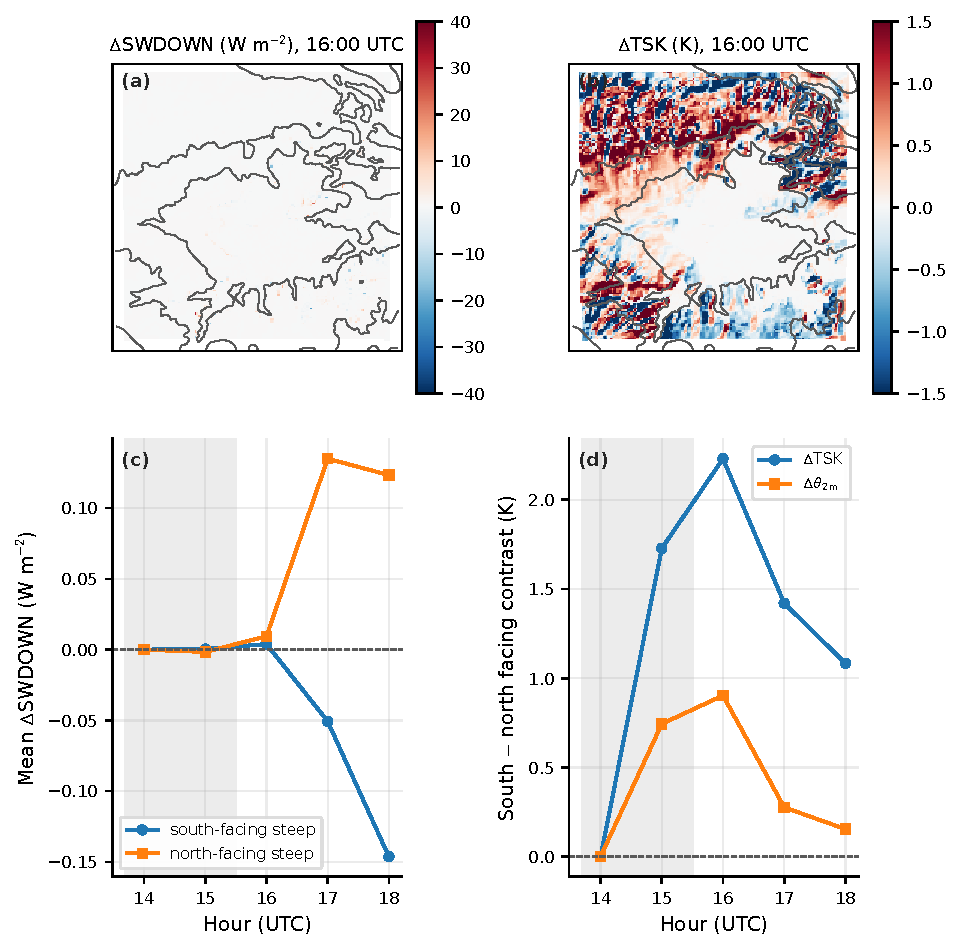
\includegraphics[width=0.88\textwidth]{verification/figures/candidates/wrf_radiation_response_cmp07_d02.pdf}%
}{\fbox{\parbox[c][0.48\textheight][c]{0.88\textwidth}{\centering Slope-aware-radiation diagnostic unavailable.}}}
\caption{Diagnostic response to slope-aware radiation and terrain shading on the controlled fine-terrain branch.
The archived flat-plane shortwave field showed negligible differences, whereas skin temperature showed an aspect-organised response on steep terrain.
The figure demonstrates that the common station metric can miss a localised model response, but it does not show that slope-aware radiation improved or degraded the cold pool and supports no configuration ranking.}
\label{fig:supp-radiation}
\end{figure}

\clearpage
\section{Within-X8 d04 Heat-Deficit Transport}
\label{sec:supp-x8-process}

X8 is a single multiply confounded context run with 111.111\,m nominal d04 grid spacing, 50 vertical levels, and 10\,min output.
The panels in Figure~\ref{fig:supp-x8-process} describe resolved model processes within X8 and do not provide a comparison, independent validation, resolution response, numerical-viability test, or basin-export estimate.

\begin{figure}[H]
\centering
\begin{minipage}[t]{0.49\textwidth}
\centering
\textbf{(a)}\\[-2pt]
\IfFileExists{verification/figures/candidates/x8_deficit_transport_map_15z.pdf}{%
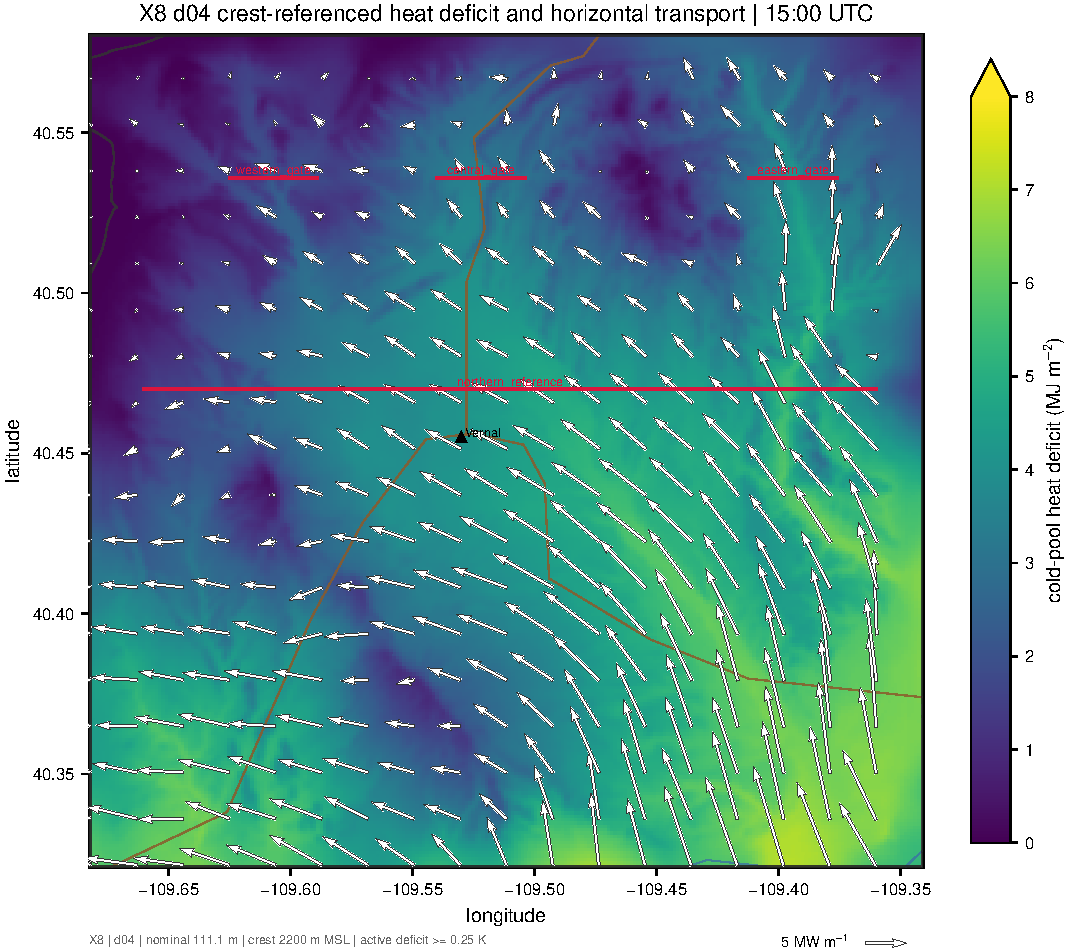
\includegraphics[width=\linewidth]{verification/figures/candidates/x8_deficit_transport_map_15z.pdf}%
}{\fbox{\parbox[c][0.27\textheight][c]{0.90\linewidth}{\centering X8 d04 heat-deficit transport map unavailable.}}}
\end{minipage}\hfill
\begin{minipage}[t]{0.49\textwidth}
\centering
\textbf{(b)}\\[-2pt]
\IfFileExists{verification/figures/candidates/x8_deficit_transport_gates_12to18.pdf}{%
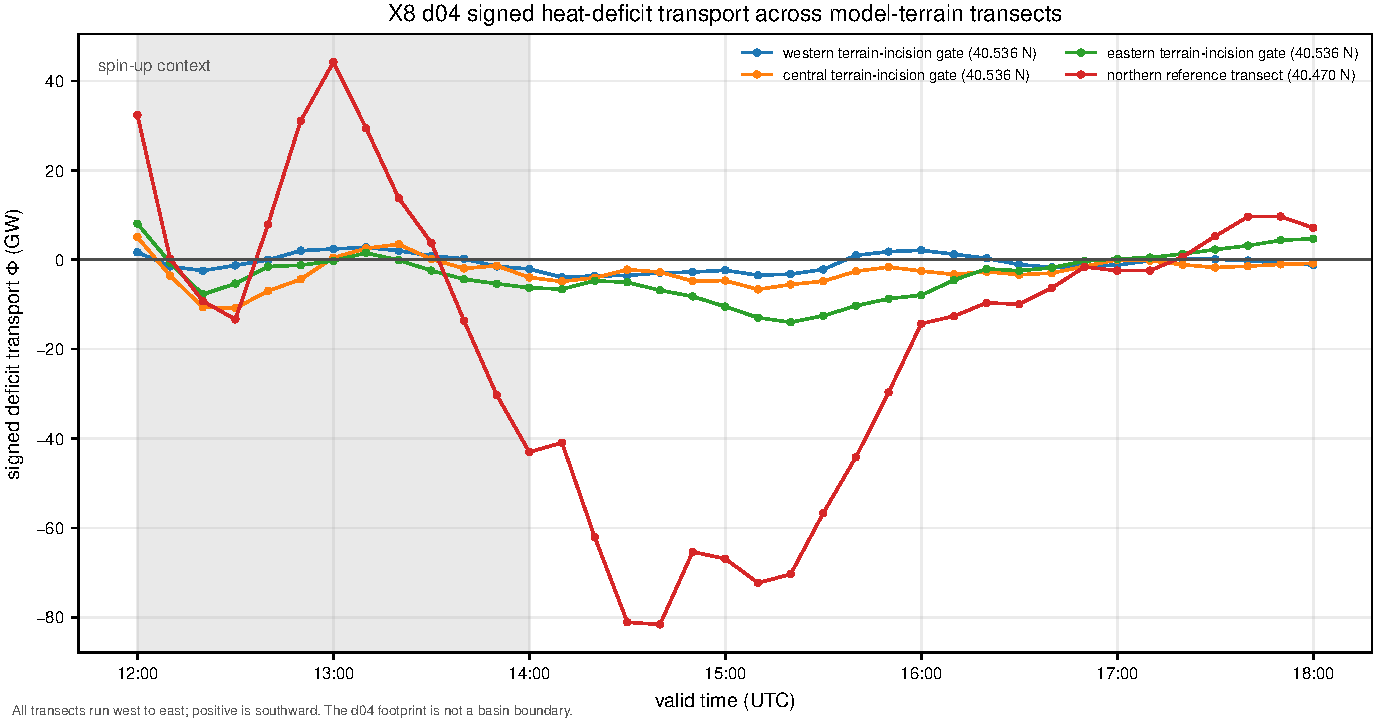
\includegraphics[width=\linewidth]{verification/figures/candidates/x8_deficit_transport_gates_12to18.pdf}%
}{\fbox{\parbox[c][0.27\textheight][c]{0.90\linewidth}{\centering X8 signed-transport series unavailable.}}}
\end{minipage}

\vspace{4pt}

\textbf{(c)}\\[-2pt]
\IfFileExists{verification/figures/candidates/x8_deficit_budget_12to18.pdf}{%
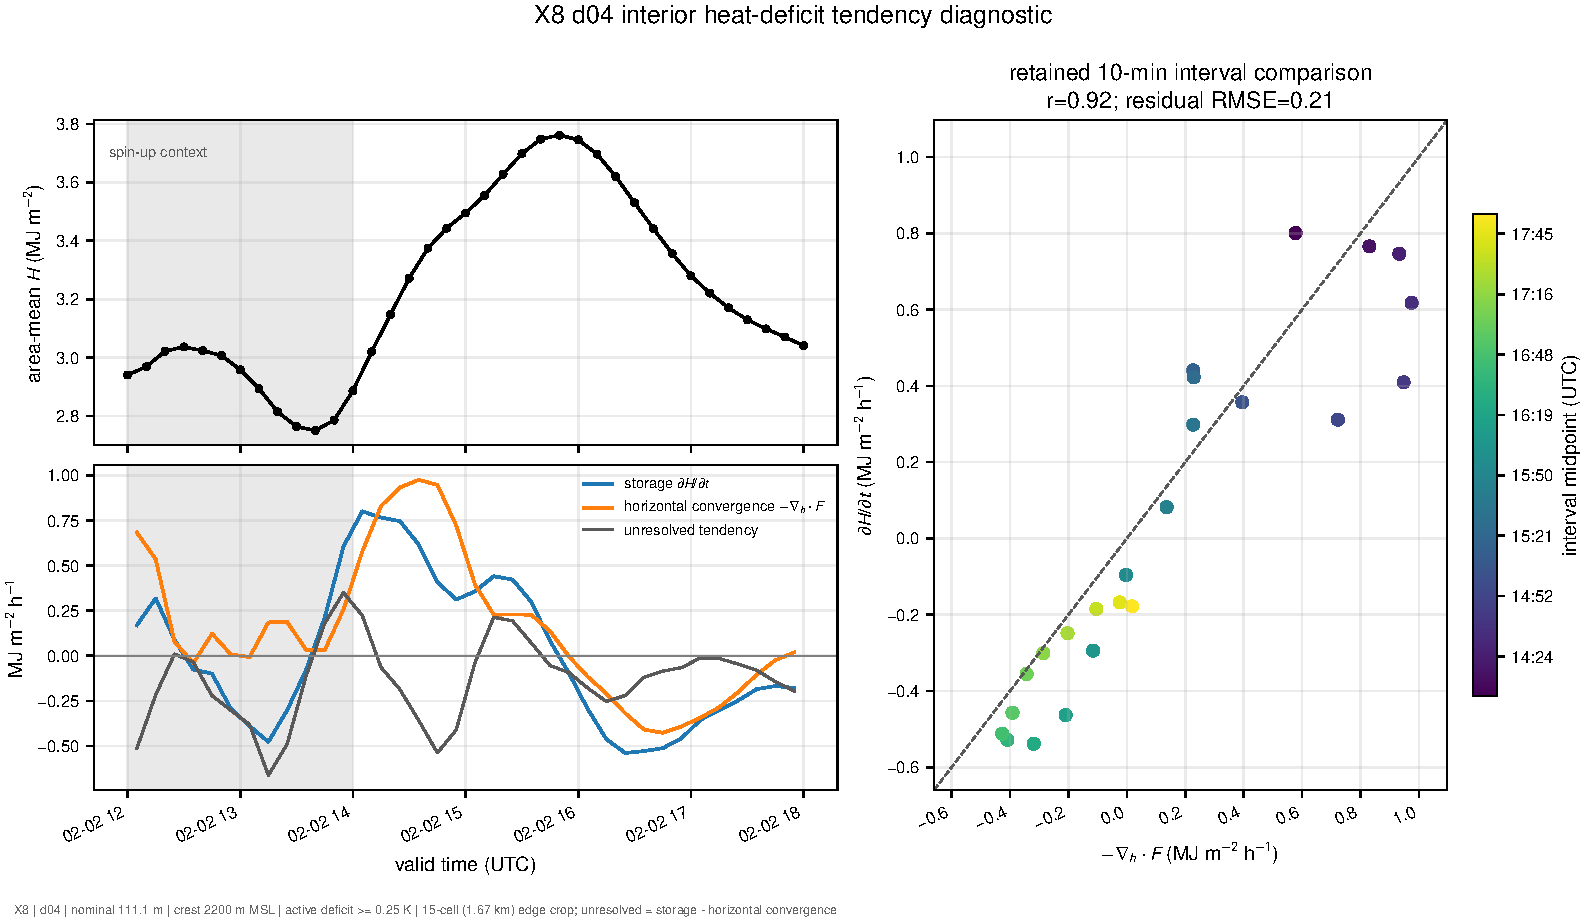
\includegraphics[width=0.90\textwidth]{verification/figures/candidates/x8_deficit_budget_12to18.pdf}%
}{\fbox{\parbox[c][0.34\textheight][c]{0.88\textwidth}{\centering X8 storage, convergence, and unresolved-tendency diagnostic unavailable.}}}
\caption{Within-X8 d04 heat-deficit transport and tendency diagnostics.
(a) Crest-referenced heat deficit $H$ and horizontal deficit transport $\mathbf{F}$ at 1500 UTC use the local potential temperature at 2200\,m mean sea level as the column reference.
The three short lines cross model-terrain incisions, while the longer line is a northern reference transect rather than a basin boundary.
(b) Signed transport at 10\,min cadence is positive southward and negative northward because every transect runs west to east.
The northern reference line reaches $-81.61$\,GW at 1440 UTC before relaxing to $+9.69$\,GW at 1750 UTC.
(c) Ten-minute finite-difference storage is compared with endpoint-mean horizontal convergence after excluding 15 cells from each d04 edge; their difference is retained as unresolved rather than attributed to a single process.
Across retained intervals, storage and horizontal convergence have $r=0.92$, while the unresolved-tendency root-mean-square error is 0.21\,MJ\,m$^{-2}$\,h$^{-1}$.
The shaded 1200--1400 UTC interval is spin-up context, and none of the panels establishes closed budget accounting, observed canyon drainage, or basin export.}
\label{fig:supp-x8-process}
\end{figure}

\end{document}
